\documentclass{beamer}
\usepackage{remreset}
\usepackage{etoolbox}
\usepackage{comment}
\usepackage{graphicx}
%\usepackage{dtklogos}
\usepackage{dsfont}
\usepackage{amsmath,amssymb}
\usepackage{tikz} 
\usepackage{cancel}
\setbeamercovered{invisible}


\makeatletter
\@removefromreset{subsection}{section}
\patchcmd{\beamer@part}{\setcounter{subsection}{0}}{}{}
\makeatother
\setcounter{subsection}{1}
\setbeamercovered{transparent}

\mode<presentation>{}
%% preamble
\title[Income Uncertainty and Consumption Dynamics]{Income Uncertainty and Consumption Dynamics}
\author{Edmund Crawley \& Andreas Kuchler}
\date[6/21/2018]{June 21, 2018}
\usetheme{Frankfurt}
\begin{document}


\frame{\titlepage}

\section{Motivation}
\setbeamercovered{invisible}
\frame
{
	\frametitle{Overview}
	1) How does household expenditure respond to income shocks?
	\begin{itemize}
		\item To transitory shocks?
		\item To permanent shocks?
	\end{itemize}
	2) How does this vary across the population?
	\begin{itemize}
		\item Across (liquid) wealth
		\item Across age
		\item Across interest rate exposure
	\end{itemize}
	Empirical evidence on 1 weak, on 2 it is VERY weak
}
\frame{
	\frametitle{How Have Consumption Responses Been Measured?}
	Three methods:
	\begin{itemize}
		\item[1] (Natural) Experiments - stimulus checks, lotteries etc
		\begin{itemize}
			\item Few true experiments, especially for permanent shocks
			\item Data limitations
		\end{itemize}
		\item[2] Ask people
		\begin{itemize}
			\item Unclear how to interpret
		\end{itemize}
		\item[3] Use covariance structure of income and consumption
		\begin{itemize}
			\item Empirical methods (until now!) have been flawed
		\end{itemize}
	\end{itemize}
	\pause
	Our contribution
	\begin{itemize}
		\item Develop a robust method based on 3
		\item Apply it to Danish registry data
\end{itemize}
The Danish data allows us to build a detailed picture of the distribution over different household characteristics
}
\frame
{
	\frametitle{Evidence on Magnitude of Consumption Response}
	\begin{center}
	\begin{tikzpicture}
	\node (img1) {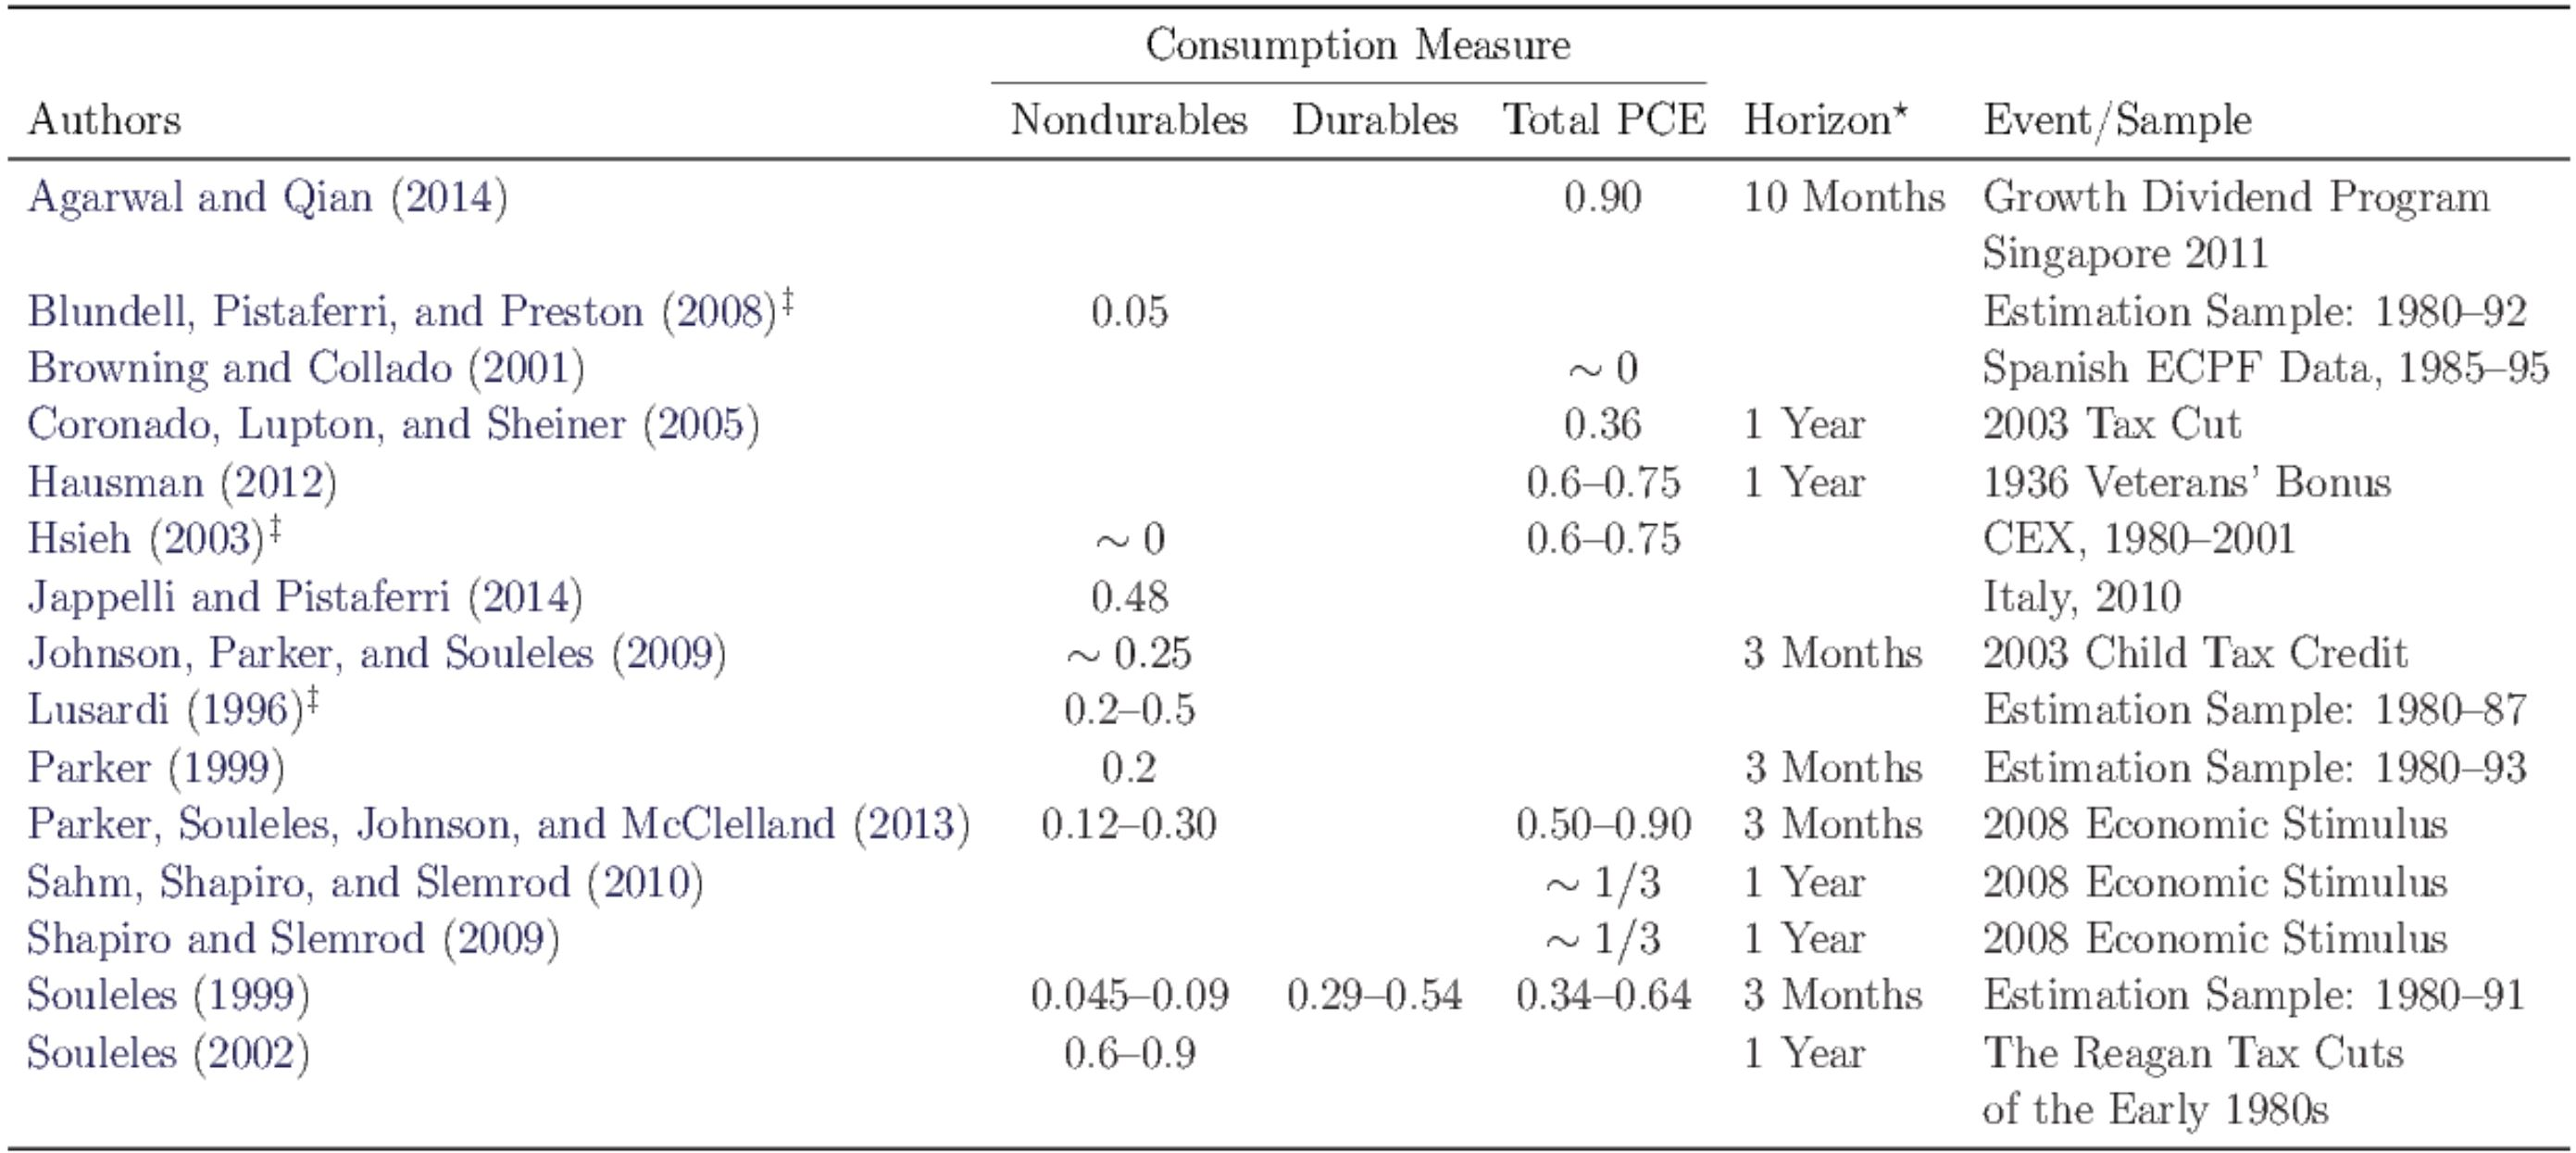
\includegraphics[height=5cm]{../Figures/MPCEmpiricalTable}};
	\end{tikzpicture}
	\tiny{Table from Carroll et al 2018}
\end{center}
Rough consensus on (3 month) MPC $\sim 30\%$
}
\frame
{
	\frametitle{Evidence on Distribution of Consumption Response}
	Auclert (2018) uses the 3 different methods to identify the distribution of MPC by unhedged interest rate exposure
	\begin{figure}
		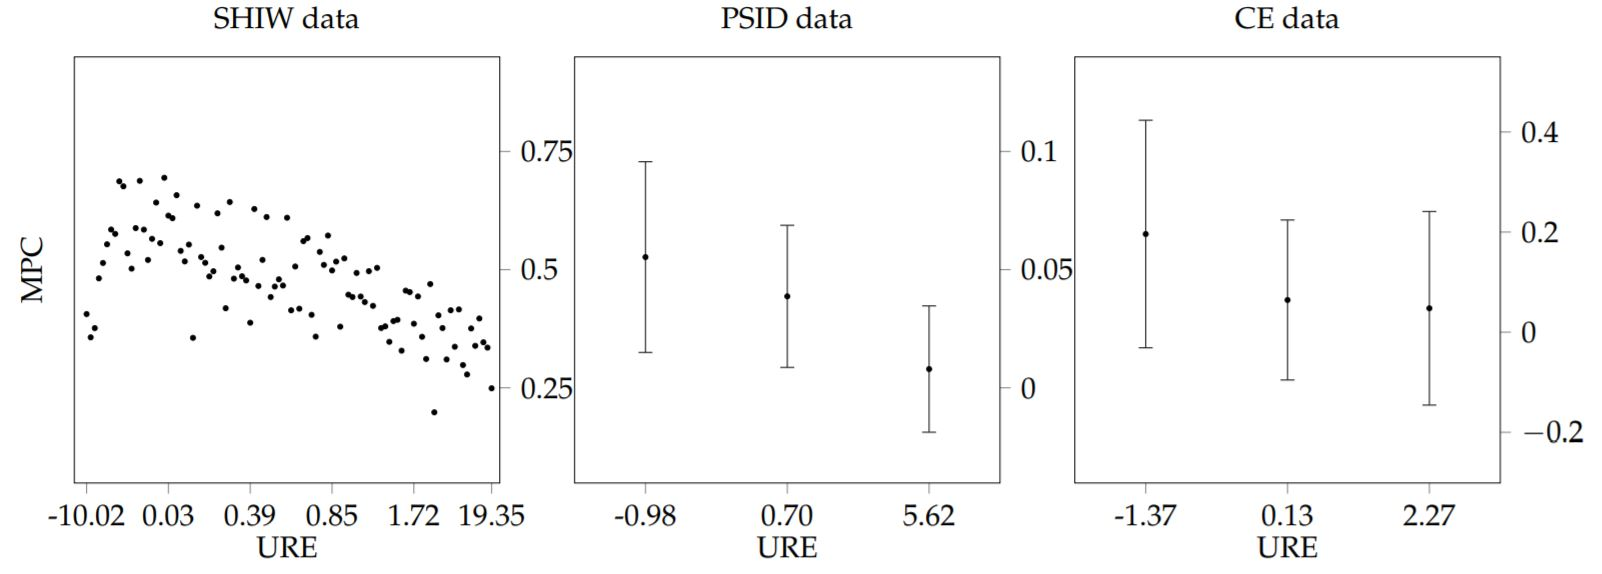
\includegraphics[scale=0.6]{../Figures/MPCDistributionAuclert}
	\end{figure}
	Recent evidence from Norwegian registry data using lottery winnings provides evidence of variation across liquid wealth
}
\frame{
	\frametitle{Results Preview}
	\begin{figure}
	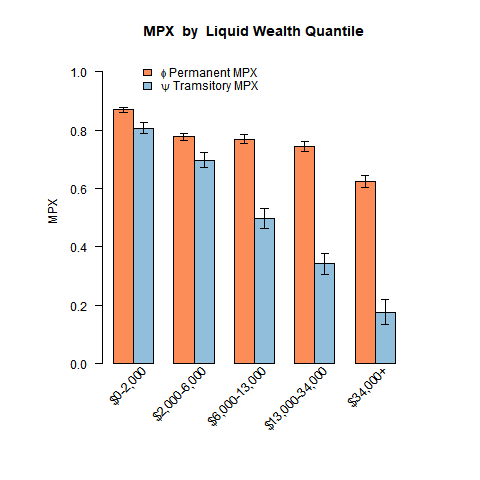
\includegraphics[scale=0.5]{../Figures/MPXByLiquidWealth_level_lincome_head.png}
	\end{figure}
}
\section{Empirical Strategy}
\setbeamercovered{invisible}
\frame
{
	\frametitle{Methodology Intuition}
	Exploit increasing importance of permanent shocks as the time over which growth is measured increases
	\begin{center}
	\begin{tikzpicture}
	\node (img1) {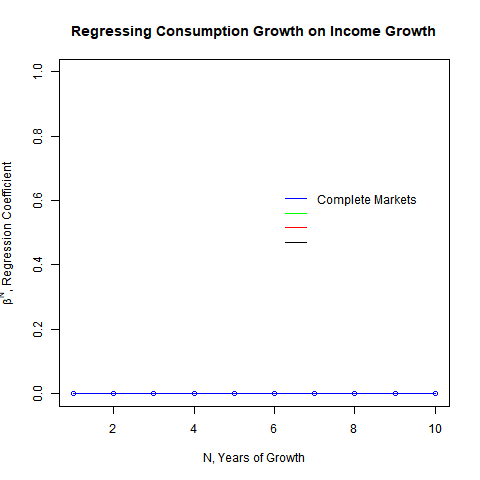
\includegraphics[height=5cm]{../Figures/basic_regression_complete_level_lincome_head.png}};
	\pause
	\node (img2) {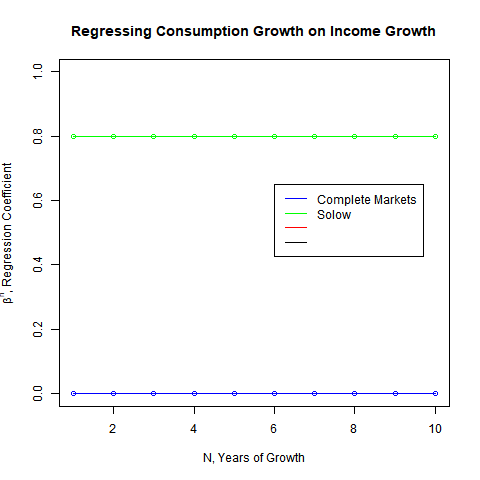
\includegraphics[height=5cm]{../Figures/basic_regression_solow_level_lincome_head.png}};
	\pause
	\node (img3) {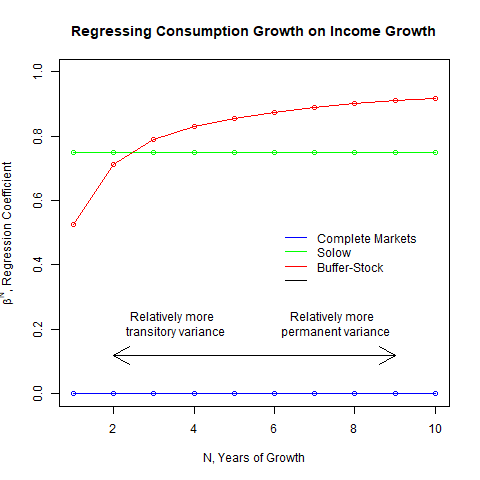
\includegraphics[height=5cm]{../Figures/basic_regression_BS_level_lincome_head.png}};
	\pause
	\node (img4) {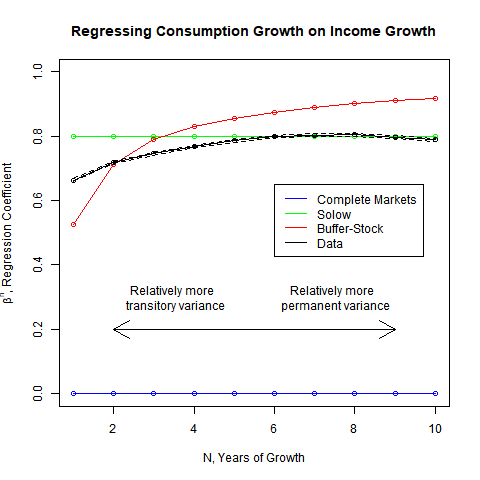
\includegraphics[height=5cm]{../Figures/basic_regression_level_lincome_head.png}};
	\end{tikzpicture}
	\end{center}
	\begin{align*}
	\Delta^N c = \beta \Delta^N y +\varepsilon
	\end{align*}
}
\frame
{
	\frametitle{Aside: Why Not Blundell, Pistaferri and Preston 2008?}
	1) Time Aggregation Problem (Crawley 2018)
	\begin{columns}
	\column{0.5\linewidth}
	\centering
	\onslide<1->{
	\begin{tikzpicture}
	\node (img1) {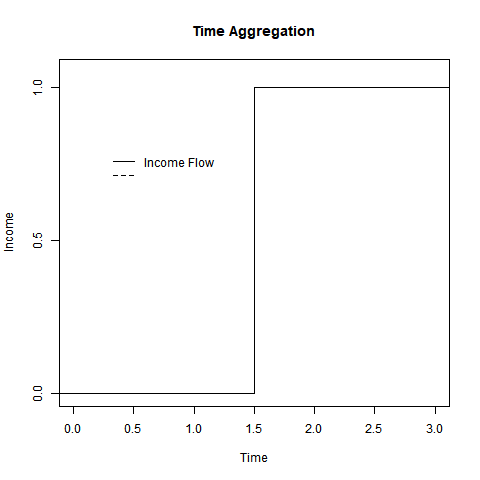
\includegraphics[height=5cm]{../Figures/TimeAggExample1.png}};
	\onslide<2->{
	\node (img2) {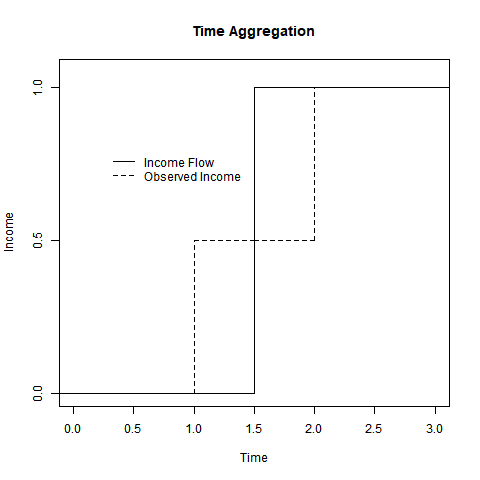
\includegraphics[height=5cm]{../Figures/TimeAggExample2.png}};
	}
	\end{tikzpicture}
	}
	\column{0.5\linewidth}
	\onslide<3->{
	PIH Example:\\
	\begin{itemize}
	\item MPC out of Permanent Shocks = 1\\
	\item MPC out of Transitory Shocks = 0\\
	\item Variances approx. equal
	\end{itemize}
	BPP method estimates MPC out of transitory shocks to be -0.6
	\end{columns}
	}
}
\frame
{
	\frametitle{Aside: Why Not Blundell, Pistaferri and Preston 2008?}
	2) BPP assume consumption is a random walk
	\begin{itemize}
		\item High transitory MPCs are incompatible with consumption following a random walk
	\end{itemize}
}
\frame
{
	\frametitle{Identification of the Income Process}
	We follow the spirit of Carroll \& Samwick (1997):\\
	\begin{itemize}
		\item Permanent income follows a random walk
		\begin{align*}
			p_t = p_{t-1} + \zeta_t
		\end{align*}
		\item Total income includes a transitory component
		\begin{align*}
			y_t = p_t +\varepsilon_t
		\end{align*}
	\end{itemize}
	Growth over N years is:
	\begin{align*}
	\Delta^N y_T &=  (\zeta_{T-N+1} + ... +\zeta_T) + \varepsilon_T - \varepsilon_{T-N} \\
	\mathrm{Var}(\Delta^N y_T) &= N\mathrm{Var}(\zeta) + 2\mathrm{Var}(\varepsilon)
	\end{align*}
}
\frame
{
	\frametitle{Identification of the Income Process}
	We follow the spirit of Carroll \& Samwick (1997):\\
	\begin{itemize}
		\item If transitory income follows an MA(2) process:
		\begin{align*}
			y_t &= p_t + \varepsilon_t + \theta_1 \varepsilon_{t-1} +\theta_2 \varepsilon_{t-2} \\
			\implies \mathrm{Var}(\Delta^N y_T) &= N\underbrace{\mathrm{Var}(\zeta)}_{\text{Perm var}} + 2\underbrace{(1+\theta_1^2+\theta_2^2)\mathrm{Var}(\varepsilon)}_{\text{``Total" trans var}} \text{ if } N\geq 3
		\end{align*}
	\end{itemize}
	Carroll \& Samwick use $N=3,4,5$ to identify permanent shock variance and ``total" transitory shock variance
	\bigskip
	\pause
	\begin{itemize}
		\item[1] How does time aggregation affect this identification?
		\item[2] What might the equivalent of ``robust to MA(2) transitory shocks" be in continuous time?
	\end{itemize}
}
\frame
{
	\frametitle{Identification of the Income Process}
	Carroll \& Samwick in Continuous Time with Aggregation\\
	\begin{itemize}
		\item To begin assume no persistence in the transitory shock
		\item $p_t$ and $q_t$ are independent martingale processes with independent increments
		\begin{align*}
			\mathrm{Var}(p_t-p_{t-1}) &= \sigma^2_p \\
			\mathrm{Var}(q_t-q_{t-1}) &= \sigma^2_q
		\end{align*}
		\item Instantaneous income is equal to the flow of permanent income plus the transitory income component
		\begin{align*}
		dy_t = p_t dt + dq_t
		\end{align*}
	\end{itemize}
	\pause
	We observe $\bar{y}_T$, total income over year $T$:
	\begin{align*}
	\bar{y}_T &= \int_{T-1}^{T}p_t dt + q_T - q_{T-1} \\
	\implies  \mathrm{Var}(\Delta^N \bar{y}_T) &= (N-\frac{1}{3})\sigma_p + 2\sigma_q
	\end{align*}
}
\frame
{
	\frametitle{Identification of the Income Process}
	Allow a generic persistence in transitory shock
	\begin{itemize}
		\item Following shock, transitory income flow decays as:
		\begin{align*}
			f(t)  \text{ where } f(t)=0 \text{ if } t>2
		\end{align*}
	\end{itemize}
	\vspace*{-0.15in}
	\begin{figure}
		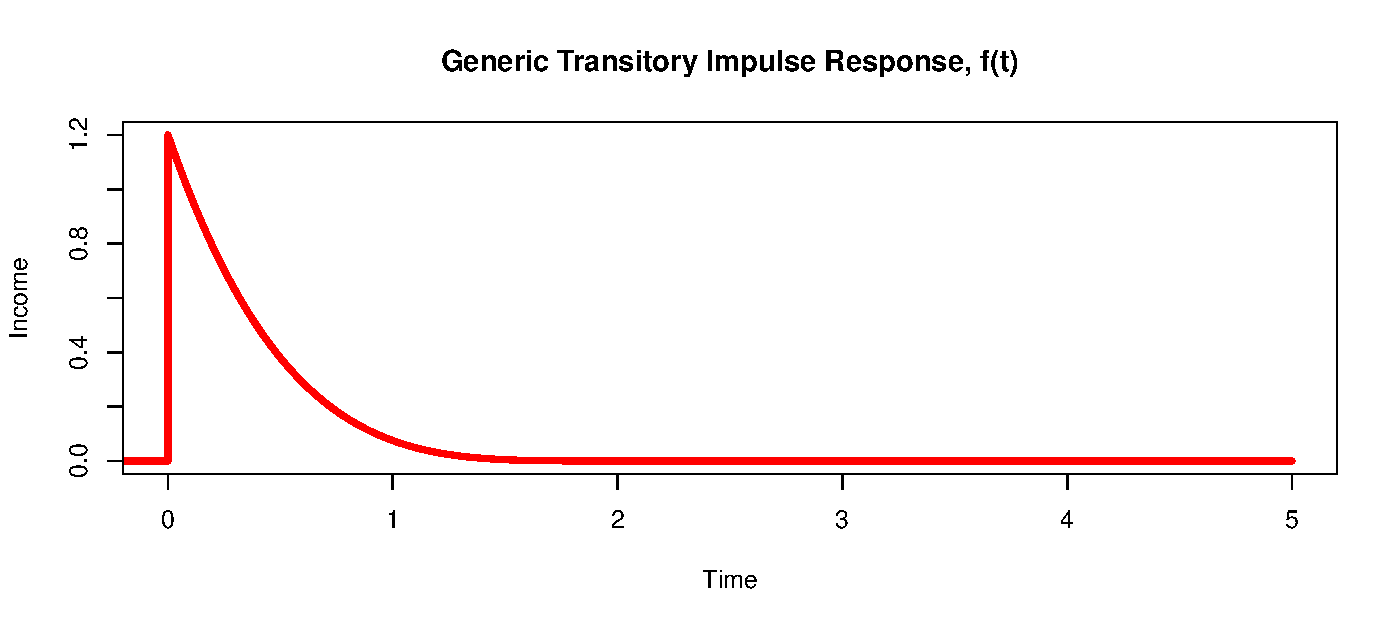
\includegraphics[scale=0.3]{../Figures/GenericTransitory.pdf}
	\end{figure}
	\vspace*{-0.15in}
	\begin{align*}
	y_t &= p_t + \int_{t-2}^{t} f(t-s)dq_s\\
	\implies \mathrm{Var}(\Delta^n \bar{y}_T) &= (n-\frac{1}{3})\sigma^2_p +  2 \sigma^2_{\tilde{q}} \text{   for }n \geq 3
	\end{align*}	
	where $	\tilde{q_T} = \int_{T-1}^{T}\int_{t-2}^{t} f(t-s)dq_s dt$ is the time aggregated transitory component of income
}
\frame
{
	\frametitle{Identification of the Consumption Response}
	Assumptions on Consumption\\
	\begin{itemize}
		\item Permanent: Consumption permanently moves by fraction $\phi$ of the income shock
		\item Transitory: Allow for generic impulse response $g(t)$ where $g(t) = 0$ for $t>2$
	\end{itemize}
	\vspace*{-0.2in}
	\begin{center}
	\begin{tikzpicture}
	\node (img1) {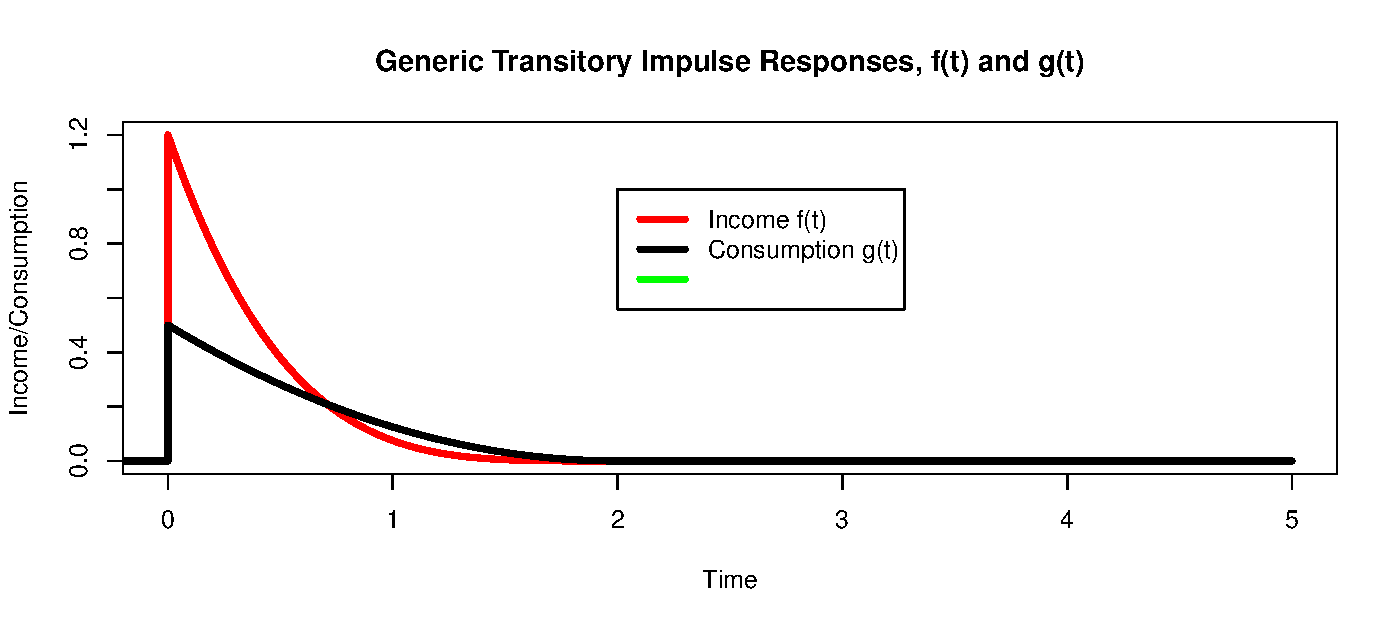
\includegraphics[height=4cm]{../Figures/GenericTransitoryConsumption.pdf}};
	\pause
	\node (img2) at (img1) {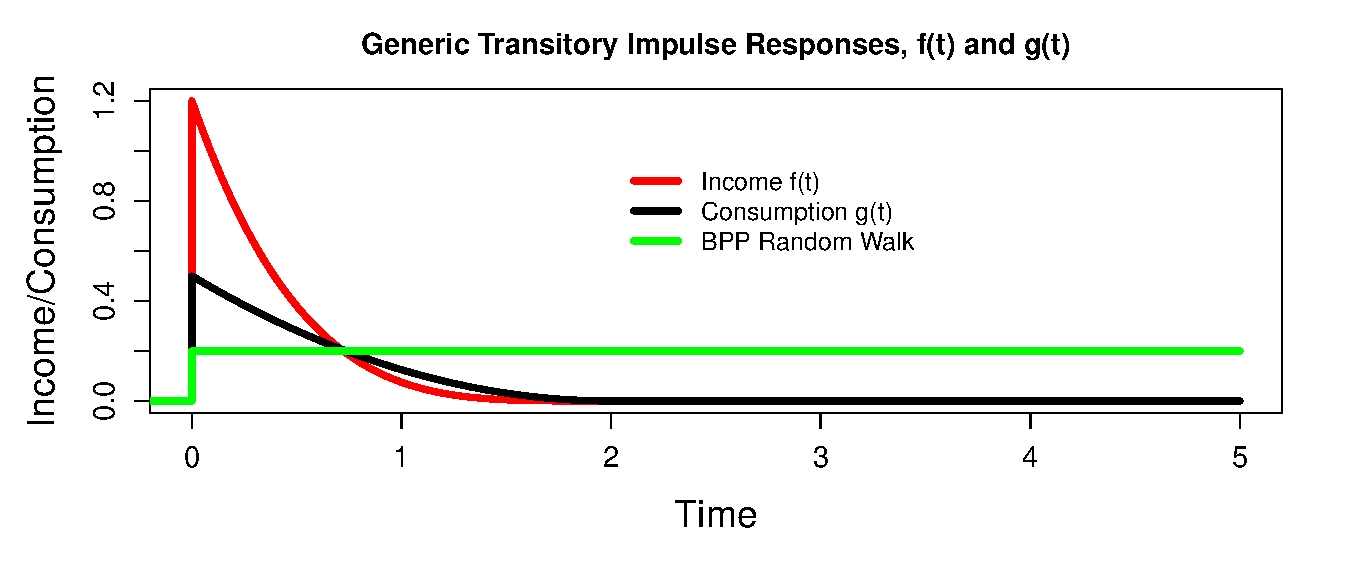
\includegraphics[height=4cm]{../Figures/GenericTransitoryConsumptionWithBPP.pdf}};
	\end{tikzpicture}
	\end{center}
	\vspace*{-0.2in}
	This is a key difference between what we assume and BPP
}
\frame
{
	\frametitle{Identification of the Consumption Response}
	Consumption flow is given by:
	\begin{align*}
	c_t  &= \phi p_t  + \int_{t-2}^{t} g(t-s)dq_s  \\
	\implies \mathrm{Cov}(\Delta^N \bar{c_T},\Delta^n \bar{y_T} ) &= \phi (N-\frac{1}{3}) \sigma^2_p + 2 \psi \sigma^2_{\tilde{q}}
	\end{align*}
	where  $\psi = \frac{\mathrm{Cov}(\tilde{c},\tilde{q})}{\mathrm{Var}(\tilde{q})}$, the regression coefficient of `transitory' consumption on transitory income \\
	\pause
	\bigskip
	\begin{itemize}
		\item $\phi$: MPX out of permanent income shocks
		\item $\psi$: MPX out of transitory income shocks
	\end{itemize}
}
\frame
{
	\frametitle{Full Identification}
We use GMM on the equations:
\begin{align*}
\mathrm{Var}(\Delta^n \bar{y_T} ) &=  (N-\frac{1}{3}) \sigma^2_p + 2  \sigma^2_{\tilde{q}} \\
\mathrm{Cov}(\Delta^N \bar{c_T},\Delta^n \bar{y_T} ) &= \phi (N-\frac{1}{3}) \sigma^2_p + 2 \psi \sigma^2_{\tilde{q}}
\end{align*}
with $N=3,4,5$ (total of six equations) to identify the four unknowns:
\begin{itemize}
	\item $\sigma^2_p$: Permanent shock variance
	\item $\sigma^2_{\tilde{q}}$: (Time aggregated) transitory shock variance
	\item $\phi$: MPX out of permanent income shocks
	\item $\psi$: MPX out of transitory income shocks
\end{itemize}
}
\section{Data}
\frame
{
	\frametitle{Data}
	\begin{itemize}
		\item Starting point: Register based micro data for all Danish households made available by Statistics Denmark
		\item Really good income data
		\begin{itemize}
			\item We use after-tax income for the household head, based on third-party reported tax data
		\end{itemize}
		\item We divide through by permanent income (mean income over all observed years) and take the residual after controlling for age, education, marital status etc. (along with interactions of these)
		\item Expenditure data imputed from income and wealth
		\begin{itemize}
			\item Deposit and brokerage accounts all third party reported
			\item Less accurate than income data
		\end{itemize}
	\end{itemize}
}
\frame
{
	\frametitle{Imputing Expenditure}
	We use the identity
		\begin{align*}
			C_t \equiv Y_t - S_t = Y_t - \Delta NW
		\end{align*}
	\begin{itemize}
		\item Works well for households with simple financial lives
		\item Main issue: Capital gains and losses
		\begin{itemize}
			\item Exclude households where methodology will not work well (eg Business owners)
			\item Exclude housing wealth and years with housing transactions
			\item Capital gains for stocks based on a diversified index
		\end{itemize}
		\item Noisy, but perhaps better than surveys (Browning and Leth-Petersen, 2003; Eika et al., 2017; Fagereng and Halvorsen, 2017; Koijen et al., 2015; Kolsrod et al., 2017; Kreiner et al., 2015)
		\item Huge sample size advantage: sample covers 23.3 million observations over 2004-2015 (approx 1.9 million per year)
	\end{itemize}
}
\section{Results}
\frame
{
	\frametitle{Shock Variance by Age}
	\begin{figure}
		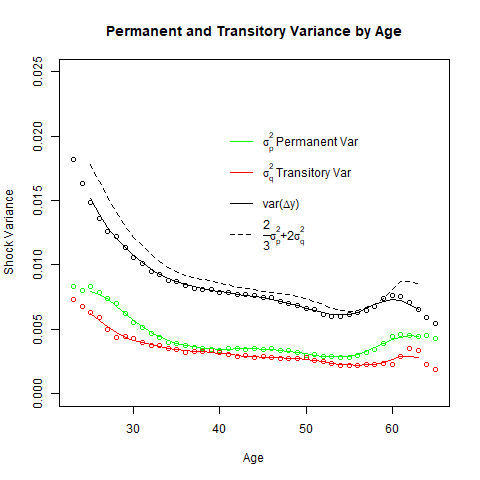
\includegraphics[scale=0.35]{../Figures/VarianceByAge_level_lincome_head.png}
	\end{figure}
	\vspace{-0.25in}
	The assumption of constant variance works reasonably well from mid-30's to retirement
}
\frame
{
	\frametitle{MPX by Age}
	\begin{columns}
		\column{0.5\linewidth}
		\centering
		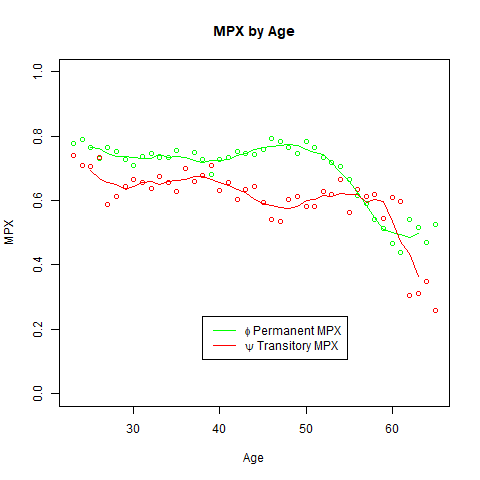
\includegraphics[scale=0.35]{../Figures/MPXByAge_level_lincome_head.png}
		\column{0.5\linewidth}
		\begin{itemize}
			\item $\phi \approx 0.8$, declines towards retirement
			\item $\psi \approx 0.5$, constant
		\end{itemize}
	\end{columns} 	
}
\frame
{
	\frametitle{MPX by Liquid Wealth}
	\begin{columns}
		\column{0.5\linewidth}
		\centering
		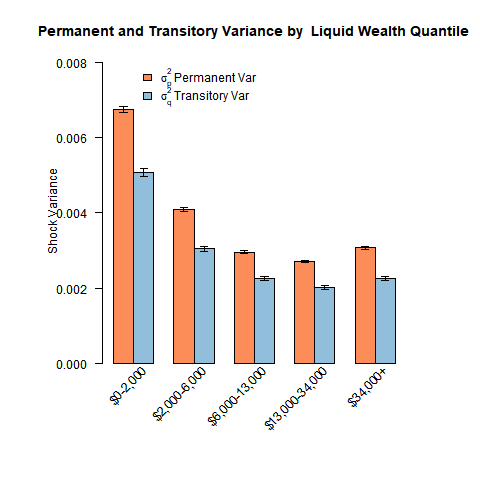
\includegraphics[scale=0.35]{../Figures/VarianceByLiquidWealth_level_lincome_head.png}
		\column{0.5\linewidth}
		\centering
		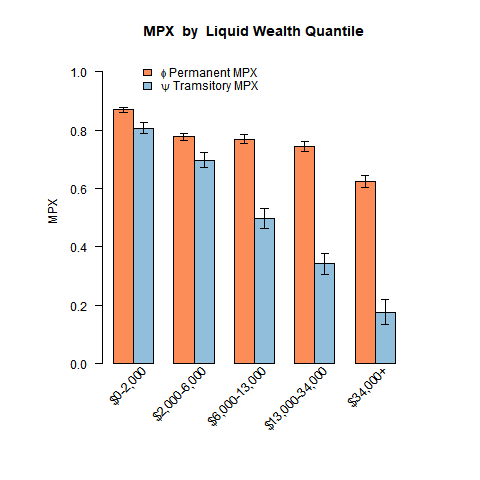
\includegraphics[scale=0.35]{../Figures/MPXByLiquidWealth_level_lincome_head.png}
	\end{columns} 	
}
\frame
{
	\frametitle{Durables}
	Our expenditure measure include ALL expenditure
	\begin{itemize}
		\item Household goods (electronics, kitchen equipment, etc)
		\item Cars
		\item Home improvements (roof repair, extensions)
	\end{itemize}
	Durables make up about 10\% of total expenditure\\
	\pause
	\bigskip
	But theory suggests durable expenditures should not be proportional to permanent income changes 
	\begin{itemize}
		\item This may bias our results
	\end{itemize}
}
\frame
{
	\frametitle{Durables}
	Suppose households \textit{instantaneously} upgrade their durable goods and then pay a constant flow of depreciation:
	\begin{align*}
	dc_t = \phi p_t dt + \color{red} \phi_{d} dp_t \color{black} + \psi dq_t
	\end{align*}
	\begin{itemize}
		\item $\phi$ can be interpreted as the MP\color{red}C \color{black}to permanent shocks, where consumption includes non-durables and the service \textit{flow} from durable goods
		\item $\phi_{d}$ is the proportion of the (annual) permanent shock that is spent instantaneously on durables
		\item $\psi$ is the MPX out of transitory income, exactly as before
	\end{itemize}
	\pause
	Then our estimates of $\phi$ and $\psi$ are unbiased. We have no way of estimating $\phi_d$
}
\frame
{
	\frametitle{Durables}
	If households act with some delay things are different. Suppose they wait 1 year
	\begin{align*}
	dc_t = \phi p_t dt + \color{red} \phi_{d} dp_{t-1} \color{black} + \psi dq_t
	\end{align*}
	\begin{itemize}
		\item $\mathbb{E}(\hat{\phi})=\phi$ Permanent MPC is unbiased
		\item $\mathbb{E}(\hat{\psi})=\psi \color{red} + \frac{\sigma^2_p}{2\sigma^2_q}\phi_d$ Transitory MPX is upward biased
	\end{itemize}
	\begin{figure}
	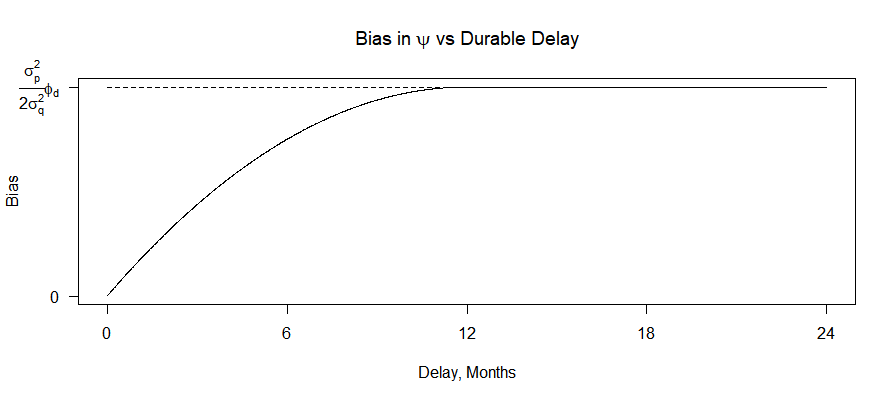
\includegraphics[scale=0.3]{../Figures/DurableBias.png}
	\end{figure}
}
\frame
{
	\frametitle{Durables}
	We have data on value of household cars\\
	\begin{itemize}
		\item Construct expenditure excluding car purchases and sales
		\begin{align*}
		C_T^{\text{nocar}} = C_T - \Delta \text{CarValue}
		\end{align*}
		\item Construct proxy for non durable consumption (Cars $\approx \frac{1}{3}$ durable expenditure)
		\begin{align*}
		C_T^{\text{nondurable}} = C_T - 3\Delta \text{CarValue}
		\end{align*}
	\end{itemize}
}
\frame
{
	\frametitle{Durables}
	\begin{center}
	\begin{tikzpicture}
	\node (img1) {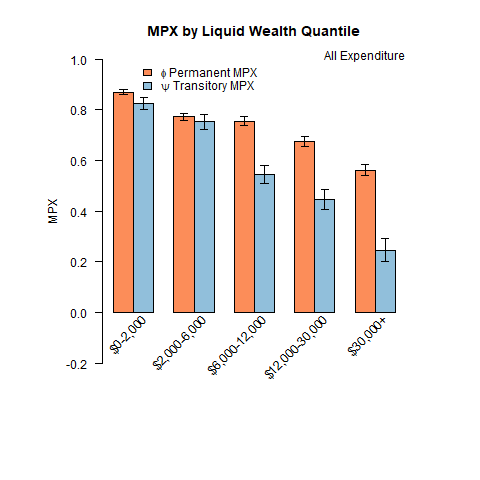
\includegraphics[scale=0.5]{../Figures/MPXByDurables_all.png}};
	\pause
	\node (img2)
	{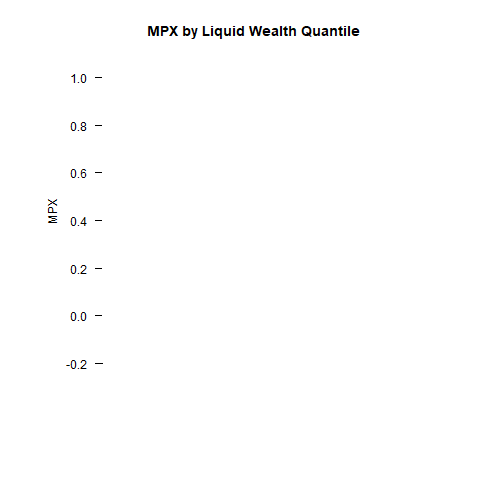
\includegraphics[scale=0.5]{../Figures/MPXByDurables_blank.png}};
	\node (img3) {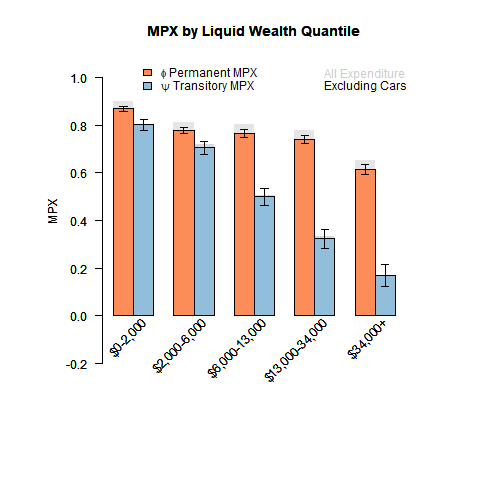
\includegraphics[scale=0.5]{../Figures/MPXByDurables_nocar.png}};
	\pause
	\node (img4)
	{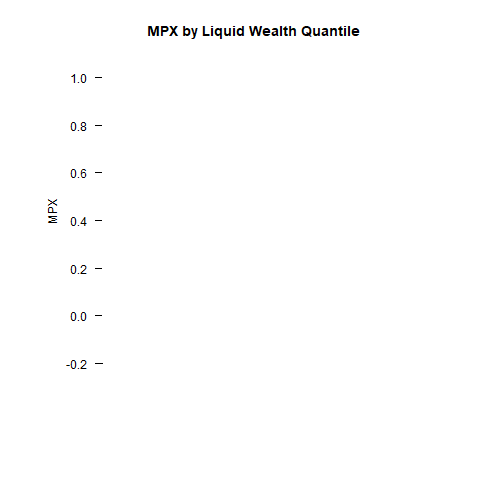
\includegraphics[scale=0.5]{../Figures/MPXByDurables_blank.png}};
	\node (img5) {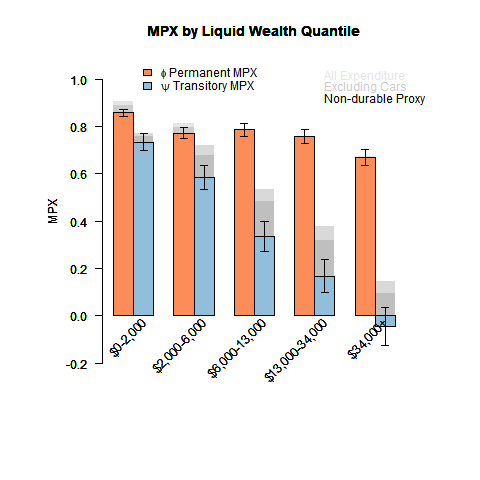
\includegraphics[scale=0.5]{../Figures/MPXByDurables_nodurableproxy.png}};
	\end{tikzpicture}
\end{center}
}
\frame
{
	\frametitle{Sensitivity to Misspecification}
	Given the MPX out of transitory and permanent income are both similar, results are not very sensitive to exact modeling assumptions
	\begin{itemize}
		\item AR(1) in permanent shock
		\item Correlation between permanent and transitory shocks
	\end{itemize}
}
\frame
{
	\frametitle{Why is Transitory MPX so large?}
	Explantion 1: It just is \\
	\bigskip
	In line with some other estimates e.g.
	\begin{itemize}
		\item Agarwal \& Quin (2014) find 90\% 10 month MPX from the 2011 Singapore Growth Dividend Program (excellent data)
		\item Parker et al. (2013) find 50-90\% 3 month MPX out of 2008 stimulus
		\item Souleles (2002) finds 60-90\% 12 month MPX out of Reagan tax cuts
	\end{itemize}
	\pause
	However, Fagereng et al (2017) find an MPX of 35\% using lottery winnings and similar expenditure data in Norway

}
\frame
{
	\frametitle{Why is Transitory MPX so large?}
	Explantion 2: Income is Endogenous\\
	\bigskip
	Potential model would need
	\begin{itemize}
		\item Permanent and transitory income uncertainty
		\item Transitory taste shocks
		\item Endogenous labor supply
	\end{itemize}
	Is a quantitatively reasonable model feasible?
	\begin{itemize}
	\item How big (or small) will labor elasticity need to be?
	\item Seems unlikely the high wealthy MPX can be matched
\end{itemize}
}
\frame
{
	\frametitle{Why is Transitory MPX so large?}
	Explantion 3: Measurement Error\\
	\bigskip
	\begin{itemize}
		\item Method is robust to \textit{classical} measurement error in expenditure
		\item Method is (mostly) robust to \textit{classical} measurement error in income
		\item The imputation method potentially introduces correlation between measurement error in income and expenditure (a problem)
	\end{itemize}
	Unobserved income uncorrelated with observed income is OK\\
	Problem if income is observed with error
}
\section{Way Forward}
\frame
{
	\frametitle{Why is Transitory MPX so large?}
	How can we dig into this?\\
	\bigskip
	\begin{itemize}
		\item Break down sources of income
		\begin{itemize}
			\item MPX from secondary earner is much higher than primary earner
			\item Look only at households who have little choice over work hours
			\item Look at wages and hours worked rather than income
		\end{itemize}	
		\item Use income data from an independent source (employer payment data)
	\end{itemize}
}
\frame
{
	\frametitle{Model}
	How will a model in which labor decisions are driven by spending needs behave over the business cycle?\\
	\begin{itemize}
		\item In a recession households have much less ability to insure themselves through their labor supply
		\item May increase saving to compensate
	\end{itemize}
}
\frame
{
	\frametitle{Model}
	GHH preferences with a taste shifter
	\begin{align*}
	u(c,l,\varphi) &= U(\varphi c - G(l))
	\end{align*}
	First order condition w.r.t $l$
	\begin{align*}
	\implies l = G^{'-1}(\varphi w)
	\end{align*}
	where $w$ is the wage\\
	\bigskip
	Note - even the wealthy adjust their labor
}
\end{document}


